\documentclass[1p]{elsarticle_modified}
%\bibliographystyle{elsarticle-num}

%\usepackage[colorlinks]{hyperref}
%\usepackage{abbrmath_seonhwa} %\Abb, \Ascr, \Acal ,\Abf, \Afrak
\usepackage{amsfonts}
\usepackage{amssymb}
\usepackage{amsmath}
\usepackage{amsthm}
\usepackage{scalefnt}
\usepackage{amsbsy}
\usepackage{kotex}
\usepackage{caption}
\usepackage{subfig}
\usepackage{color}
\usepackage{graphicx}
\usepackage{xcolor} %% white, black, red, green, blue, cyan, magenta, yellow
\usepackage{float}
\usepackage{setspace}
\usepackage{hyperref}

\usepackage{tikz}
\usetikzlibrary{arrows}

\usepackage{multirow}
\usepackage{array} % fixed length table
\usepackage{hhline}

%%%%%%%%%%%%%%%%%%%%%
\makeatletter
\renewcommand*\env@matrix[1][\arraystretch]{%
	\edef\arraystretch{#1}%
	\hskip -\arraycolsep
	\let\@ifnextchar\new@ifnextchar
	\array{*\c@MaxMatrixCols c}}
\makeatother %https://tex.stackexchange.com/questions/14071/how-can-i-increase-the-line-spacing-in-a-matrix
%%%%%%%%%%%%%%%

\usepackage[normalem]{ulem}

\newcommand{\msout}[1]{\ifmmode\text{\sout{\ensuremath{#1}}}\else\sout{#1}\fi}
%SOURCE: \msout is \stkout macro in https://tex.stackexchange.com/questions/20609/strikeout-in-math-mode

\newcommand{\cancel}[1]{
	\ifmmode
	{\color{red}\msout{#1}}
	\else
	{\color{red}\sout{#1}}
	\fi
}

\newcommand{\add}[1]{
	{\color{blue}\uwave{#1}}
}

\newcommand{\replace}[2]{
	\ifmmode
	{\color{red}\msout{#1}}{\color{blue}\uwave{#2}}
	\else
	{\color{red}\sout{#1}}{\color{blue}\uwave{#2}}
	\fi
}

\newcommand{\Sol}{\mathcal{S}} %segment
\newcommand{\D}{D} %diagram
\newcommand{\A}{\mathcal{A}} %arc


%%%%%%%%%%%%%%%%%%%%%%%%%%%%%5 test

\def\sl{\operatorname{\textup{SL}}(2,\Cbb)}
\def\psl{\operatorname{\textup{PSL}}(2,\Cbb)}
\def\quan{\mkern 1mu \triangleright \mkern 1mu}

\theoremstyle{definition}
\newtheorem{thm}{Theorem}[section]
\newtheorem{prop}[thm]{Proposition}
\newtheorem{lem}[thm]{Lemma}
\newtheorem{ques}[thm]{Question}
\newtheorem{cor}[thm]{Corollary}
\newtheorem{defn}[thm]{Definition}
\newtheorem{exam}[thm]{Example}
\newtheorem{rmk}[thm]{Remark}
\newtheorem{alg}[thm]{Algorithm}

\newcommand{\I}{\sqrt{-1}}
\begin{document}

%\begin{frontmatter}
%
%\title{Boundary parabolic representations of knots up to 8 crossings}
%
%%% Group authors per affiliation:
%\author{Yunhi Cho} 
%\address{Department of Mathematics, University of Seoul, Seoul, Korea}
%\ead{yhcho@uos.ac.kr}
%
%
%\author{Seonhwa Kim} %\fnref{s_kim}}
%\address{Center for Geometry and Physics, Institute for Basic Science, Pohang, 37673, Korea}
%\ead{ryeona17@ibs.re.kr}
%
%\author{Hyuk Kim}
%\address{Department of Mathematical Sciences, Seoul National University, Seoul 08826, Korea}
%\ead{hyukkim@snu.ac.kr}
%
%\author{Seokbeom Yoon}
%\address{Department of Mathematical Sciences, Seoul National University, Seoul, 08826,  Korea}
%\ead{sbyoon15@snu.ac.kr}
%
%\begin{abstract}
%We find all boundary parabolic representation of knots up to 8 crossings.
%
%\end{abstract}
%\begin{keyword}
%    \MSC[2010] 57M25 
%\end{keyword}
%
%\end{frontmatter}

%\linenumbers
%\tableofcontents
%
\newcommand\colored[1]{\textcolor{white}{\rule[-0.35ex]{0.8em}{1.4ex}}\kern-0.8em\color{red} #1}%
%\newcommand\colored[1]{\textcolor{white}{ #1}\kern-2.17ex	\textcolor{white}{ #1}\kern-1.81ex	\textcolor{white}{ #1}\kern-2.15ex\color{red}#1	}

{\Large $\underline{12n_{0788}~(K12n_{0788})}$}

\setlength{\tabcolsep}{10pt}
\renewcommand{\arraystretch}{1.6}
\vspace{1cm}\begin{tabular}{m{100pt}>{\centering\arraybackslash}m{274pt}}
\multirow{5}{120pt}{
	\centering
	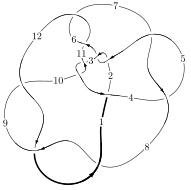
\includegraphics[width=112pt]{../../../GIT/diagram.site/Diagrams/png/2877_12n_0788.png}\\
\ \ \ A knot diagram\footnotemark}&
\allowdisplaybreaks
\textbf{Linearized knot diagam} \\
\cline{2-2}
 &
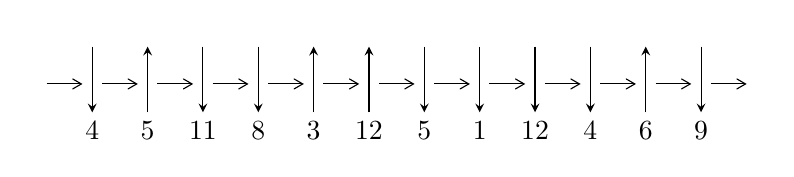
\begin{tikzpicture}[x=20pt, y=17pt]
	% nodes
	\node (C0) at (0, 0) {};
	\node (C1) at (1, 0) {};
	\node (C1U) at (1, +1) {};
	\node (C1D) at (1, -1) {4};

	\node (C2) at (2, 0) {};
	\node (C2U) at (2, +1) {};
	\node (C2D) at (2, -1) {5};

	\node (C3) at (3, 0) {};
	\node (C3U) at (3, +1) {};
	\node (C3D) at (3, -1) {11};

	\node (C4) at (4, 0) {};
	\node (C4U) at (4, +1) {};
	\node (C4D) at (4, -1) {8};

	\node (C5) at (5, 0) {};
	\node (C5U) at (5, +1) {};
	\node (C5D) at (5, -1) {3};

	\node (C6) at (6, 0) {};
	\node (C6U) at (6, +1) {};
	\node (C6D) at (6, -1) {12};

	\node (C7) at (7, 0) {};
	\node (C7U) at (7, +1) {};
	\node (C7D) at (7, -1) {5};

	\node (C8) at (8, 0) {};
	\node (C8U) at (8, +1) {};
	\node (C8D) at (8, -1) {1};

	\node (C9) at (9, 0) {};
	\node (C9U) at (9, +1) {};
	\node (C9D) at (9, -1) {12};

	\node (C10) at (10, 0) {};
	\node (C10U) at (10, +1) {};
	\node (C10D) at (10, -1) {4};

	\node (C11) at (11, 0) {};
	\node (C11U) at (11, +1) {};
	\node (C11D) at (11, -1) {6};

	\node (C12) at (12, 0) {};
	\node (C12U) at (12, +1) {};
	\node (C12D) at (12, -1) {9};
	\node (C13) at (13, 0) {};

	% arrows
	\draw[->,>={angle 60}]
	(C0) edge (C1) (C1) edge (C2) (C2) edge (C3) (C3) edge (C4) (C4) edge (C5) (C5) edge (C6) (C6) edge (C7) (C7) edge (C8) (C8) edge (C9) (C9) edge (C10) (C10) edge (C11) (C11) edge (C12) (C12) edge (C13) ;	\draw[->,>=stealth]
	(C1U) edge (C1D) (C2D) edge (C2U) (C3U) edge (C3D) (C4U) edge (C4D) (C5D) edge (C5U) (C6D) edge (C6U) (C7U) edge (C7D) (C8U) edge (C8D) (C9U) edge (C9D) (C10U) edge (C10D) (C11D) edge (C11U) (C12U) edge (C12D) ;
	\end{tikzpicture} \\
\hhline{~~} \\& 
\textbf{Solving Sequence} \\ \cline{2-2} 
 &
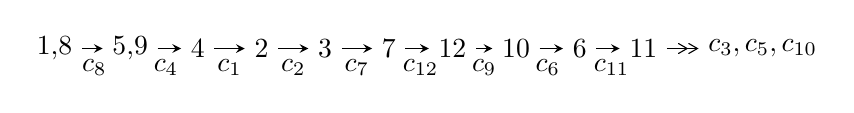
\begin{tikzpicture}[x=23pt, y=7pt]
	% node
	\node (A0) at (-1/8, 0) {1,8};
	\node (A1) at (17/16, 0) {5,9};
	\node (A2) at (17/8, 0) {4};
	\node (A3) at (25/8, 0) {2};
	\node (A4) at (33/8, 0) {3};
	\node (A5) at (41/8, 0) {7};
	\node (A6) at (49/8, 0) {12};
	\node (A7) at (57/8, 0) {10};
	\node (A8) at (65/8, 0) {6};
	\node (A9) at (73/8, 0) {11};
	\node (C1) at (1/2, -1) {$c_{8}$};
	\node (C2) at (13/8, -1) {$c_{4}$};
	\node (C3) at (21/8, -1) {$c_{1}$};
	\node (C4) at (29/8, -1) {$c_{2}$};
	\node (C5) at (37/8, -1) {$c_{7}$};
	\node (C6) at (45/8, -1) {$c_{12}$};
	\node (C7) at (53/8, -1) {$c_{9}$};
	\node (C8) at (61/8, -1) {$c_{6}$};
	\node (C9) at (69/8, -1) {$c_{11}$};
	\node (A10) at (11, 0) {$c_{3},c_{5},c_{10}$};

	% edge
	\draw[->,>=stealth]	
	(A0) edge (A1) (A1) edge (A2) (A2) edge (A3) (A3) edge (A4) (A4) edge (A5) (A5) edge (A6) (A6) edge (A7) (A7) edge (A8) (A8) edge (A9) ;
	\draw[->>,>={angle 60}]	
	(A9) edge (A10);
\end{tikzpicture} \\ 

\end{tabular} \\

\footnotetext{
The image of knot diagram is generated by the software ``\textbf{Draw programme}" developed by Andrew Bartholomew(\url{http://www.layer8.co.uk/maths/draw/index.htm\#Running-draw}), where we modified some parts for our purpose(\url{https://github.com/CATsTAILs/LinksPainter}).
}\phantom \\ \newline 
\centering \textbf{Ideals for irreducible components\footnotemark of $X_{\text{par}}$} 
 
\begin{align*}
I^u_{1}&=\langle 
1.58578\times10^{94} u^{73}+3.02439\times10^{94} u^{72}+\cdots+7.24165\times10^{94} b-1.13790\times10^{95},\\
\phantom{I^u_{1}}&\phantom{= \langle  }6.83460\times10^{94} u^{73}+2.06996\times10^{95} u^{72}+\cdots+7.24165\times10^{94} a-1.20278\times10^{96},\;u^{74}+3 u^{73}+\cdots+21 u+1\rangle \\
I^u_{2}&=\langle 
- u^{18}+3 u^{17}+\cdots+b-1,\;u^{19}- u^{18}+\cdots+a+3,\;u^{20}-2 u^{19}+\cdots+11 u^2+1\rangle \\
\\
\end{align*}
\raggedright * 2 irreducible components of $\dim_{\mathbb{C}}=0$, with total 94 representations.\\
\footnotetext{All coefficients of polynomials are rational numbers. But the coefficients are sometimes approximated in decimal forms when there is not enough margin.}
\newpage
\renewcommand{\arraystretch}{1}
\centering \section*{I. $I^u_{1}= \langle 1.59\times10^{94} u^{73}+3.02\times10^{94} u^{72}+\cdots+7.24\times10^{94} b-1.14\times10^{95},\;6.83\times10^{94} u^{73}+2.07\times10^{95} u^{72}+\cdots+7.24\times10^{94} a-1.20\times10^{96},\;u^{74}+3 u^{73}+\cdots+21 u+1 \rangle$}
\flushleft \textbf{(i) Arc colorings}\\
\begin{tabular}{m{7pt} m{180pt} m{7pt} m{180pt} }
\flushright $a_{1}=$&$\begin{pmatrix}0\\u\end{pmatrix}$ \\
\flushright $a_{8}=$&$\begin{pmatrix}1\\0\end{pmatrix}$ \\
\flushright $a_{5}=$&$\begin{pmatrix}-0.943790 u^{73}-2.85841 u^{72}+\cdots-200.219 u+16.6092\\-0.218980 u^{73}-0.417638 u^{72}+\cdots+27.3920 u+1.57132\end{pmatrix}$ \\
\flushright $a_{9}=$&$\begin{pmatrix}1\\u^2\end{pmatrix}$ \\
\flushright $a_{4}=$&$\begin{pmatrix}-1.16277 u^{73}-3.27605 u^{72}+\cdots-172.827 u+18.1805\\-0.218980 u^{73}-0.417638 u^{72}+\cdots+27.3920 u+1.57132\end{pmatrix}$ \\
\flushright $a_{2}=$&$\begin{pmatrix}-3.74724 u^{73}-11.5498 u^{72}+\cdots-1374.87 u-47.8329\\-0.289918 u^{73}-0.893819 u^{72}+\cdots-5.30721 u+1.13701\end{pmatrix}$ \\
\flushright $a_{3}=$&$\begin{pmatrix}0.150555 u^{73}+0.0467585 u^{72}+\cdots-582.950 u-39.8482\\-0.519493 u^{73}-1.69333 u^{72}+\cdots-12.9835 u-0.00334082\end{pmatrix}$ \\
\flushright $a_{7}=$&$\begin{pmatrix}-1.09362 u^{73}-3.80737 u^{72}+\cdots-462.305 u-29.4024\\-0.0433920 u^{73}+0.106412 u^{72}+\cdots-6.49614 u+0.217922\end{pmatrix}$ \\
\flushright $a_{12}=$&$\begin{pmatrix}u\\u^3+u\end{pmatrix}$ \\
\flushright $a_{10}=$&$\begin{pmatrix}u^2+1\\u^4+2 u^2\end{pmatrix}$ \\
\flushright $a_{6}=$&$\begin{pmatrix}-1.24781 u^{73}-4.44356 u^{72}+\cdots-463.401 u-29.5039\\0.0832740 u^{73}+0.529036 u^{72}+\cdots-3.79157 u+0.290107\end{pmatrix}$ \\
\flushright $a_{11}=$&$\begin{pmatrix}1.06428 u^{73}+2.50104 u^{72}+\cdots+542.210 u+39.2751\\-0.0130542 u^{73}+0.238478 u^{72}+\cdots+15.1776 u+0.0881159\end{pmatrix}$\\&\end{tabular}
\flushleft \textbf{(ii) Obstruction class $= -1$}\\~\\
\flushleft \textbf{(iii) Cusp Shapes $= 0.346623 u^{73}+2.28437 u^{72}+\cdots+298.542 u+13.6537$}\\~\\
\newpage\renewcommand{\arraystretch}{1}
\flushleft \textbf{(iv) u-Polynomials at the component}\newline \\
\begin{tabular}{m{50pt}|m{274pt}}
Crossings & \hspace{64pt}u-Polynomials at each crossing \\
\hline $$\begin{aligned}c_{1}\end{aligned}$$&$\begin{aligned}
&u^{74}-12 u^{73}+\cdots+512 u+73
\end{aligned}$\\
\hline $$\begin{aligned}c_{2},c_{5}\end{aligned}$$&$\begin{aligned}
&u^{74}-22 u^{72}+\cdots+12106 u+4059
\end{aligned}$\\
\hline $$\begin{aligned}c_{3},c_{10}\end{aligned}$$&$\begin{aligned}
&u^{74}- u^{73}+\cdots+18411 u+6049
\end{aligned}$\\
\hline $$\begin{aligned}c_{4},c_{7}\end{aligned}$$&$\begin{aligned}
&u^{74}-4 u^{73}+\cdots-2438 u+529
\end{aligned}$\\
\hline $$\begin{aligned}c_{6},c_{11}\end{aligned}$$&$\begin{aligned}
&u^{74}- u^{73}+\cdots-1273 u+2357
\end{aligned}$\\
\hline $$\begin{aligned}c_{8},c_{9},c_{12}\end{aligned}$$&$\begin{aligned}
&u^{74}-3 u^{73}+\cdots-21 u+1
\end{aligned}$\\
\hline
\end{tabular}\\~\\
\newpage\renewcommand{\arraystretch}{1}
\flushleft \textbf{(v) Riley Polynomials at the component}\newline \\
\begin{tabular}{m{50pt}|m{274pt}}
Crossings & \hspace{64pt}Riley Polynomials at each crossing \\
\hline $$\begin{aligned}c_{1}\end{aligned}$$&$\begin{aligned}
&y^{74}+46 y^{72}+\cdots+277034 y+5329
\end{aligned}$\\
\hline $$\begin{aligned}c_{2},c_{5}\end{aligned}$$&$\begin{aligned}
&y^{74}-44 y^{73}+\cdots-265207924 y+16475481
\end{aligned}$\\
\hline $$\begin{aligned}c_{3},c_{10}\end{aligned}$$&$\begin{aligned}
&y^{74}+47 y^{73}+\cdots+954117711 y+36590401
\end{aligned}$\\
\hline $$\begin{aligned}c_{4},c_{7}\end{aligned}$$&$\begin{aligned}
&y^{74}+36 y^{73}+\cdots+5248738 y+279841
\end{aligned}$\\
\hline $$\begin{aligned}c_{6},c_{11}\end{aligned}$$&$\begin{aligned}
&y^{74}-45 y^{73}+\cdots-110160379 y+5555449
\end{aligned}$\\
\hline $$\begin{aligned}c_{8},c_{9},c_{12}\end{aligned}$$&$\begin{aligned}
&y^{74}+69 y^{73}+\cdots+273 y+1
\end{aligned}$\\
\hline
\end{tabular}\\~\\
\newpage\flushleft \textbf{(vi) Complex Volumes and Cusp Shapes}
$$\begin{array}{c|c|c}  
\text{Solutions to }I^u_{1}& \I (\text{vol} + \sqrt{-1}CS) & \text{Cusp shape}\\
 \hline 
\begin{aligned}
u &= -0.936804 + 0.339968 I \\
a &= \phantom{-}0.622927 + 0.688917 I \\
b &= \phantom{-}0.710500 - 1.130150 I\end{aligned}
 & \phantom{-}2.76516 + 11.24560 I & \phantom{-0.000000 } 0 \\ \hline\begin{aligned}
u &= -0.936804 - 0.339968 I \\
a &= \phantom{-}0.622927 - 0.688917 I \\
b &= \phantom{-}0.710500 + 1.130150 I\end{aligned}
 & \phantom{-}2.76516 - 11.24560 I & \phantom{-0.000000 } 0 \\ \hline\begin{aligned}
u &= \phantom{-}0.930090 + 0.208950 I \\
a &= -0.334369 + 0.260725 I \\
b &= -0.663146 - 0.942118 I\end{aligned}
 & -0.61830 - 4.53833 I & \phantom{-0.000000 } 0 \\ \hline\begin{aligned}
u &= \phantom{-}0.930090 - 0.208950 I \\
a &= -0.334369 - 0.260725 I \\
b &= -0.663146 + 0.942118 I\end{aligned}
 & -0.61830 + 4.53833 I & \phantom{-0.000000 } 0 \\ \hline\begin{aligned}
u &= -0.319333 + 1.020450 I \\
a &= \phantom{-}0.23353 + 1.63070 I \\
b &= \phantom{-}0.553683 - 0.674115 I\end{aligned}
 & \phantom{-}3.67304 - 1.08231 I & \phantom{-0.000000 } 0 \\ \hline\begin{aligned}
u &= -0.319333 - 1.020450 I \\
a &= \phantom{-}0.23353 - 1.63070 I \\
b &= \phantom{-}0.553683 + 0.674115 I\end{aligned}
 & \phantom{-}3.67304 + 1.08231 I & \phantom{-0.000000 } 0 \\ \hline\begin{aligned}
u &= -0.069737 + 1.104620 I \\
a &= \phantom{-}0.46995 + 1.52306 I \\
b &= \phantom{-}0.315493 - 0.757914 I\end{aligned}
 & \phantom{-}3.55481 - 1.00960 I & \phantom{-0.000000 } 0 \\ \hline\begin{aligned}
u &= -0.069737 - 1.104620 I \\
a &= \phantom{-}0.46995 - 1.52306 I \\
b &= \phantom{-}0.315493 + 0.757914 I\end{aligned}
 & \phantom{-}3.55481 + 1.00960 I & \phantom{-0.000000 } 0 \\ \hline\begin{aligned}
u &= -0.064033 + 0.874740 I \\
a &= \phantom{-}0.598935 + 0.016465 I \\
b &= -0.805267 - 0.384169 I\end{aligned}
 & -0.142484 - 0.979938 I & -4.00000 + 2.35513 I \\ \hline\begin{aligned}
u &= -0.064033 - 0.874740 I \\
a &= \phantom{-}0.598935 - 0.016465 I \\
b &= -0.805267 + 0.384169 I\end{aligned}
 & -0.142484 + 0.979938 I & -4.00000 - 2.35513 I\\
 \hline 
 \end{array}$$\newpage$$\begin{array}{c|c|c}  
\text{Solutions to }I^u_{1}& \I (\text{vol} + \sqrt{-1}CS) & \text{Cusp shape}\\
 \hline 
\begin{aligned}
u &= -0.738642 + 0.887199 I \\
a &= -0.557382 - 0.422145 I \\
b &= \phantom{-}0.566445 + 0.940150 I\end{aligned}
 & \phantom{-}4.40806 - 5.59603 I & \phantom{-0.000000 } 0 \\ \hline\begin{aligned}
u &= -0.738642 - 0.887199 I \\
a &= -0.557382 + 0.422145 I \\
b &= \phantom{-}0.566445 - 0.940150 I\end{aligned}
 & \phantom{-}4.40806 + 5.59603 I & \phantom{-0.000000 } 0 \\ \hline\begin{aligned}
u &= \phantom{-}0.828888 + 0.091510 I \\
a &= \phantom{-}0.737287 - 0.641900 I \\
b &= \phantom{-}0.572058 + 1.134930 I\end{aligned}
 & -0.10298 - 4.06471 I & -0.40205 + 4.72845 I \\ \hline\begin{aligned}
u &= \phantom{-}0.828888 - 0.091510 I \\
a &= \phantom{-}0.737287 + 0.641900 I \\
b &= \phantom{-}0.572058 - 1.134930 I\end{aligned}
 & -0.10298 + 4.06471 I & -0.40205 - 4.72845 I \\ \hline\begin{aligned}
u &= \phantom{-}0.789984 + 0.155180 I \\
a &= \phantom{-}0.697528 - 0.295007 I \\
b &= \phantom{-}0.608961 + 0.489624 I\end{aligned}
 & -2.13816 - 0.67532 I & -4.89240 - 0.69754 I \\ \hline\begin{aligned}
u &= \phantom{-}0.789984 - 0.155180 I \\
a &= \phantom{-}0.697528 + 0.295007 I \\
b &= \phantom{-}0.608961 - 0.489624 I\end{aligned}
 & -2.13816 + 0.67532 I & -4.89240 + 0.69754 I \\ \hline\begin{aligned}
u &= \phantom{-}0.395613 + 1.128880 I \\
a &= -0.468940 + 0.976139 I \\
b &= \phantom{-}0.587115 - 0.916327 I\end{aligned}
 & \phantom{-}3.10666 - 0.34724 I & \phantom{-0.000000 } 0 \\ \hline\begin{aligned}
u &= \phantom{-}0.395613 - 1.128880 I \\
a &= -0.468940 - 0.976139 I \\
b &= \phantom{-}0.587115 + 0.916327 I\end{aligned}
 & \phantom{-}3.10666 + 0.34724 I & \phantom{-0.000000 } 0 \\ \hline\begin{aligned}
u &= \phantom{-}0.386320 + 1.141930 I \\
a &= -0.257479 - 0.302102 I \\
b &= \phantom{-}0.741571 - 0.155531 I\end{aligned}
 & \phantom{-}0.88149 - 3.55827 I & \phantom{-0.000000 } 0 \\ \hline\begin{aligned}
u &= \phantom{-}0.386320 - 1.141930 I \\
a &= -0.257479 + 0.302102 I \\
b &= \phantom{-}0.741571 + 0.155531 I\end{aligned}
 & \phantom{-}0.88149 + 3.55827 I & \phantom{-0.000000 } 0\\
 \hline 
 \end{array}$$\newpage$$\begin{array}{c|c|c}  
\text{Solutions to }I^u_{1}& \I (\text{vol} + \sqrt{-1}CS) & \text{Cusp shape}\\
 \hline 
\begin{aligned}
u &= -0.781957 + 0.127588 I \\
a &= \phantom{-}0.468419 - 0.340993 I \\
b &= \phantom{-}0.969908 + 0.496154 I\end{aligned}
 & \phantom{-}0.83489 + 5.14638 I & -2.92699 - 4.12698 I \\ \hline\begin{aligned}
u &= -0.781957 - 0.127588 I \\
a &= \phantom{-}0.468419 + 0.340993 I \\
b &= \phantom{-}0.969908 - 0.496154 I\end{aligned}
 & \phantom{-}0.83489 - 5.14638 I & -2.92699 + 4.12698 I \\ \hline\begin{aligned}
u &= -0.690960 + 0.376818 I \\
a &= -0.930716 - 0.945879 I \\
b &= -0.790965 + 0.838168 I\end{aligned}
 & -1.32937 + 4.37262 I & -1.68695 - 7.55471 I \\ \hline\begin{aligned}
u &= -0.690960 - 0.376818 I \\
a &= -0.930716 + 0.945879 I \\
b &= -0.790965 - 0.838168 I\end{aligned}
 & -1.32937 - 4.37262 I & -1.68695 + 7.55471 I \\ \hline\begin{aligned}
u &= \phantom{-}0.208976 + 1.238970 I \\
a &= \phantom{-}0.725780 - 0.430028 I \\
b &= -1.33074 + 0.55805 I\end{aligned}
 & \phantom{-}2.07909 - 2.04945 I & \phantom{-0.000000 } 0 \\ \hline\begin{aligned}
u &= \phantom{-}0.208976 - 1.238970 I \\
a &= \phantom{-}0.725780 + 0.430028 I \\
b &= -1.33074 - 0.55805 I\end{aligned}
 & \phantom{-}2.07909 + 2.04945 I & \phantom{-0.000000 } 0 \\ \hline\begin{aligned}
u &= -0.239083 + 1.235520 I \\
a &= -0.56305 - 1.99635 I \\
b &= -0.653467 + 1.183850 I\end{aligned}
 & \phantom{-}2.21691 + 4.57437 I & \phantom{-0.000000 } 0 \\ \hline\begin{aligned}
u &= -0.239083 - 1.235520 I \\
a &= -0.56305 + 1.99635 I \\
b &= -0.653467 - 1.183850 I\end{aligned}
 & \phantom{-}2.21691 - 4.57437 I & \phantom{-0.000000 } 0 \\ \hline\begin{aligned}
u &= -0.098165 + 1.270860 I \\
a &= \phantom{-}0.22331 + 3.15689 I \\
b &= -0.02511 - 1.52128 I\end{aligned}
 & \phantom{-}11.61620 - 0.14821 I & \phantom{-0.000000 } 0 \\ \hline\begin{aligned}
u &= -0.098165 - 1.270860 I \\
a &= \phantom{-}0.22331 - 3.15689 I \\
b &= -0.02511 + 1.52128 I\end{aligned}
 & \phantom{-}11.61620 + 0.14821 I & \phantom{-0.000000 } 0\\
 \hline 
 \end{array}$$\newpage$$\begin{array}{c|c|c}  
\text{Solutions to }I^u_{1}& \I (\text{vol} + \sqrt{-1}CS) & \text{Cusp shape}\\
 \hline 
\begin{aligned}
u &= -0.290096 + 1.244670 I \\
a &= -1.42838 - 0.42517 I \\
b &= -0.079374 + 0.951986 I\end{aligned}
 & \phantom{-}9.54324 + 4.38718 I & \phantom{-0.000000 } 0 \\ \hline\begin{aligned}
u &= -0.290096 - 1.244670 I \\
a &= -1.42838 + 0.42517 I \\
b &= -0.079374 - 0.951986 I\end{aligned}
 & \phantom{-}9.54324 - 4.38718 I & \phantom{-0.000000 } 0 \\ \hline\begin{aligned}
u &= \phantom{-}0.664261 + 1.105320 I \\
a &= \phantom{-}0.578989 - 0.326355 I \\
b &= -0.309901 + 0.732892 I\end{aligned}
 & \phantom{-}1.98668 - 0.96963 I & \phantom{-0.000000 } 0 \\ \hline\begin{aligned}
u &= \phantom{-}0.664261 - 1.105320 I \\
a &= \phantom{-}0.578989 + 0.326355 I \\
b &= -0.309901 - 0.732892 I\end{aligned}
 & \phantom{-}1.98668 + 0.96963 I & \phantom{-0.000000 } 0 \\ \hline\begin{aligned}
u &= -0.703470 + 0.069064 I \\
a &= \phantom{-}0.078771 - 1.020400 I \\
b &= \phantom{-}0.318672 - 0.907573 I\end{aligned}
 & \phantom{-}5.93010 - 0.78432 I & \phantom{-}1.48301 - 0.85749 I \\ \hline\begin{aligned}
u &= -0.703470 - 0.069064 I \\
a &= \phantom{-}0.078771 + 1.020400 I \\
b &= \phantom{-}0.318672 + 0.907573 I\end{aligned}
 & \phantom{-}5.93010 + 0.78432 I & \phantom{-}1.48301 + 0.85749 I \\ \hline\begin{aligned}
u &= \phantom{-}0.000271 + 1.298230 I \\
a &= -1.73564 + 1.88420 I \\
b &= -0.120936 - 0.853354 I\end{aligned}
 & \phantom{-}9.15293 + 3.49758 I & \phantom{-0.000000 } 0 \\ \hline\begin{aligned}
u &= \phantom{-}0.000271 - 1.298230 I \\
a &= -1.73564 - 1.88420 I \\
b &= -0.120936 + 0.853354 I\end{aligned}
 & \phantom{-}9.15293 - 3.49758 I & \phantom{-0.000000 } 0 \\ \hline\begin{aligned}
u &= -0.654738 + 0.139993 I \\
a &= -0.365809 - 0.113721 I \\
b &= -0.749123 - 0.884451 I\end{aligned}
 & -1.17142 - 1.41028 I & -0.82219 - 1.94292 I \\ \hline\begin{aligned}
u &= -0.654738 - 0.139993 I \\
a &= -0.365809 + 0.113721 I \\
b &= -0.749123 + 0.884451 I\end{aligned}
 & -1.17142 + 1.41028 I & -0.82219 + 1.94292 I\\
 \hline 
 \end{array}$$\newpage$$\begin{array}{c|c|c}  
\text{Solutions to }I^u_{1}& \I (\text{vol} + \sqrt{-1}CS) & \text{Cusp shape}\\
 \hline 
\begin{aligned}
u &= -0.021534 + 1.337130 I \\
a &= \phantom{-}0.554741 - 0.978134 I \\
b &= \phantom{-}0.795121 + 0.856242 I\end{aligned}
 & \phantom{-}9.72603 - 3.20768 I & \phantom{-0.000000 } 0 \\ \hline\begin{aligned}
u &= -0.021534 - 1.337130 I \\
a &= \phantom{-}0.554741 + 0.978134 I \\
b &= \phantom{-}0.795121 - 0.856242 I\end{aligned}
 & \phantom{-}9.72603 + 3.20768 I & \phantom{-0.000000 } 0 \\ \hline\begin{aligned}
u &= -0.104300 + 1.333230 I \\
a &= -0.26774 - 2.22250 I \\
b &= \phantom{-}0.24396 + 1.72146 I\end{aligned}
 & \phantom{-}12.48010 + 3.12382 I & \phantom{-0.000000 } 0 \\ \hline\begin{aligned}
u &= -0.104300 - 1.333230 I \\
a &= -0.26774 + 2.22250 I \\
b &= \phantom{-}0.24396 - 1.72146 I\end{aligned}
 & \phantom{-}12.48010 - 3.12382 I & \phantom{-0.000000 } 0 \\ \hline\begin{aligned}
u &= -0.276951 + 1.318390 I \\
a &= \phantom{-}0.405659 + 0.960983 I \\
b &= \phantom{-}0.727988 - 1.027740 I\end{aligned}
 & \phantom{-}10.30720 + 2.74116 I & \phantom{-0.000000 } 0 \\ \hline\begin{aligned}
u &= -0.276951 - 1.318390 I \\
a &= \phantom{-}0.405659 - 0.960983 I \\
b &= \phantom{-}0.727988 + 1.027740 I\end{aligned}
 & \phantom{-}10.30720 - 2.74116 I & \phantom{-0.000000 } 0 \\ \hline\begin{aligned}
u &= \phantom{-}0.616600 + 0.149646 I \\
a &= -0.576417 + 1.181130 I \\
b &= -0.763533 - 0.734900 I\end{aligned}
 & -1.25932 - 0.85009 I & -2.93324 - 0.64796 I \\ \hline\begin{aligned}
u &= \phantom{-}0.616600 - 0.149646 I \\
a &= -0.576417 - 1.181130 I \\
b &= -0.763533 + 0.734900 I\end{aligned}
 & -1.25932 + 0.85009 I & -2.93324 + 0.64796 I \\ \hline\begin{aligned}
u &= \phantom{-}0.359175 + 1.322210 I \\
a &= \phantom{-}0.82697 - 2.18712 I \\
b &= \phantom{-}0.498014 + 1.278840 I\end{aligned}
 & \phantom{-}4.31927 - 8.33215 I & \phantom{-0.000000 } 0 \\ \hline\begin{aligned}
u &= \phantom{-}0.359175 - 1.322210 I \\
a &= \phantom{-}0.82697 + 2.18712 I \\
b &= \phantom{-}0.498014 - 1.278840 I\end{aligned}
 & \phantom{-}4.31927 + 8.33215 I & \phantom{-0.000000 } 0\\
 \hline 
 \end{array}$$\newpage$$\begin{array}{c|c|c}  
\text{Solutions to }I^u_{1}& \I (\text{vol} + \sqrt{-1}CS) & \text{Cusp shape}\\
 \hline 
\begin{aligned}
u &= -0.331105 + 1.339680 I \\
a &= -0.749942 + 0.054369 I \\
b &= \phantom{-}1.238930 + 0.313660 I\end{aligned}
 & \phantom{-}5.44209 + 9.16208 I & \phantom{-0.000000 } 0 \\ \hline\begin{aligned}
u &= -0.331105 - 1.339680 I \\
a &= -0.749942 - 0.054369 I \\
b &= \phantom{-}1.238930 - 0.313660 I\end{aligned}
 & \phantom{-}5.44209 - 9.16208 I & \phantom{-0.000000 } 0 \\ \hline\begin{aligned}
u &= -0.305381 + 1.368770 I \\
a &= \phantom{-}0.761541 + 0.467536 I \\
b &= -0.853662 - 0.650481 I\end{aligned}
 & \phantom{-}3.67876 + 2.15533 I & \phantom{-0.000000 } 0 \\ \hline\begin{aligned}
u &= -0.305381 - 1.368770 I \\
a &= \phantom{-}0.761541 - 0.467536 I \\
b &= -0.853662 + 0.650481 I\end{aligned}
 & \phantom{-}3.67876 - 2.15533 I & \phantom{-0.000000 } 0 \\ \hline\begin{aligned}
u &= \phantom{-}0.275962 + 1.383250 I \\
a &= -0.15950 + 2.10027 I \\
b &= -0.462021 - 1.121230 I\end{aligned}
 & \phantom{-}3.68775 - 4.15450 I & \phantom{-0.000000 } 0 \\ \hline\begin{aligned}
u &= \phantom{-}0.275962 - 1.383250 I \\
a &= -0.15950 - 2.10027 I \\
b &= -0.462021 + 1.121230 I\end{aligned}
 & \phantom{-}3.68775 + 4.15450 I & \phantom{-0.000000 } 0 \\ \hline\begin{aligned}
u &= \phantom{-}0.34603 + 1.39240 I \\
a &= \phantom{-}0.49266 - 1.38993 I \\
b &= \phantom{-}0.540130 + 0.835161 I\end{aligned}
 & \phantom{-}2.80424 - 4.78161 I & \phantom{-0.000000 } 0 \\ \hline\begin{aligned}
u &= \phantom{-}0.34603 - 1.39240 I \\
a &= \phantom{-}0.49266 + 1.38993 I \\
b &= \phantom{-}0.540130 - 0.835161 I\end{aligned}
 & \phantom{-}2.80424 + 4.78161 I & \phantom{-0.000000 } 0 \\ \hline\begin{aligned}
u &= \phantom{-}0.39339 + 1.39442 I \\
a &= -0.31063 + 1.63356 I \\
b &= -0.77536 - 1.22079 I\end{aligned}
 & \phantom{-}4.43148 - 9.25628 I & \phantom{-0.000000 } 0 \\ \hline\begin{aligned}
u &= \phantom{-}0.39339 - 1.39442 I \\
a &= -0.31063 - 1.63356 I \\
b &= -0.77536 + 1.22079 I\end{aligned}
 & \phantom{-}4.43148 + 9.25628 I & \phantom{-0.000000 } 0\\
 \hline 
 \end{array}$$\newpage$$\begin{array}{c|c|c}  
\text{Solutions to }I^u_{1}& \I (\text{vol} + \sqrt{-1}CS) & \text{Cusp shape}\\
 \hline 
\begin{aligned}
u &= -0.27655 + 1.49326 I \\
a &= -0.28891 - 1.91776 I \\
b &= -0.713564 + 1.014530 I\end{aligned}
 & \phantom{-}4.77334 + 7.96569 I & \phantom{-0.000000 } 0 \\ \hline\begin{aligned}
u &= -0.27655 - 1.49326 I \\
a &= -0.28891 + 1.91776 I \\
b &= -0.713564 - 1.014530 I\end{aligned}
 & \phantom{-}4.77334 - 7.96569 I & \phantom{-0.000000 } 0 \\ \hline\begin{aligned}
u &= -0.38358 + 1.47124 I \\
a &= \phantom{-}0.47036 + 1.92708 I \\
b &= \phantom{-}0.72193 - 1.29934 I\end{aligned}
 & \phantom{-}8.5275 + 16.0127 I & \phantom{-0.000000 } 0 \\ \hline\begin{aligned}
u &= -0.38358 - 1.47124 I \\
a &= \phantom{-}0.47036 - 1.92708 I \\
b &= \phantom{-}0.72193 + 1.29934 I\end{aligned}
 & \phantom{-}8.5275 - 16.0127 I & \phantom{-0.000000 } 0 \\ \hline\begin{aligned}
u &= \phantom{-}0.049778 + 0.404950 I \\
a &= \phantom{-}1.039240 + 0.230406 I \\
b &= -0.504136 - 0.382867 I\end{aligned}
 & -0.230831 - 1.075800 I & -3.86726 + 5.56314 I \\ \hline\begin{aligned}
u &= \phantom{-}0.049778 - 0.404950 I \\
a &= \phantom{-}1.039240 - 0.230406 I \\
b &= -0.504136 + 0.382867 I\end{aligned}
 & -0.230831 + 1.075800 I & -3.86726 - 5.56314 I \\ \hline\begin{aligned}
u &= -0.00897 + 1.65353 I \\
a &= -0.17869 + 1.83789 I \\
b &= \phantom{-}0.212633 - 0.762848 I\end{aligned}
 & \phantom{-}12.84880 - 0.51128 I & \phantom{-0.000000 } 0 \\ \hline\begin{aligned}
u &= -0.00897 - 1.65353 I \\
a &= -0.17869 - 1.83789 I \\
b &= \phantom{-}0.212633 + 0.762848 I\end{aligned}
 & \phantom{-}12.84880 + 0.51128 I & \phantom{-0.000000 } 0 \\ \hline\begin{aligned}
u &= -0.318578 + 0.088858 I \\
a &= \phantom{-}1.46832 - 0.71391 I \\
b &= \phantom{-}0.12577 + 1.49843 I\end{aligned}
 & \phantom{-}7.89983 + 1.60233 I & -5.43520 - 6.25438 I \\ \hline\begin{aligned}
u &= -0.318578 - 0.088858 I \\
a &= \phantom{-}1.46832 + 0.71391 I \\
b &= \phantom{-}0.12577 - 1.49843 I\end{aligned}
 & \phantom{-}7.89983 - 1.60233 I & -5.43520 + 6.25438 I\\
 \hline 
 \end{array}$$\newpage$$\begin{array}{c|c|c}  
\text{Solutions to }I^u_{1}& \I (\text{vol} + \sqrt{-1}CS) & \text{Cusp shape}\\
 \hline 
\begin{aligned}
u &= -0.10261 + 1.70630 I \\
a &= -0.280005 - 1.271740 I \\
b &= \phantom{-}0.219435 + 0.960300 I\end{aligned}
 & \phantom{-}13.66950 - 2.42291 I & \phantom{-0.000000 } 0 \\ \hline\begin{aligned}
u &= -0.10261 - 1.70630 I \\
a &= -0.280005 + 1.271740 I \\
b &= \phantom{-}0.219435 - 0.960300 I\end{aligned}
 & \phantom{-}13.66950 + 2.42291 I & \phantom{-0.000000 } 0 \\ \hline\begin{aligned}
u &= -0.0287687 + 0.0617431 I \\
a &= \phantom{-}26.4987 - 3.7687 I \\
b &= \phantom{-}0.331976 + 0.710871 I\end{aligned}
 & \phantom{-}5.14104 - 3.45109 I & \phantom{-}1.82404 + 12.33527 I \\ \hline\begin{aligned}
u &= -0.0287687 - 0.0617431 I \\
a &= \phantom{-}26.4987 + 3.7687 I \\
b &= \phantom{-}0.331976 - 0.710871 I\end{aligned}
 & \phantom{-}5.14104 + 3.45109 I & \phantom{-}1.82404 - 12.33527 I\\
 \hline 
 \end{array}$$\newpage\newpage\renewcommand{\arraystretch}{1}
\centering \section*{II. $I^u_{2}= \langle - u^{18}+3 u^{17}+\cdots+b-1,\;u^{19}- u^{18}+\cdots+a+3,\;u^{20}-2 u^{19}+\cdots+11 u^2+1 \rangle$}
\flushleft \textbf{(i) Arc colorings}\\
\begin{tabular}{m{7pt} m{180pt} m{7pt} m{180pt} }
\flushright $a_{1}=$&$\begin{pmatrix}0\\u\end{pmatrix}$ \\
\flushright $a_{8}=$&$\begin{pmatrix}1\\0\end{pmatrix}$ \\
\flushright $a_{5}=$&$\begin{pmatrix}- u^{19}+u^{18}+\cdots+u-3\\u^{18}-3 u^{17}+\cdots-5 u+1\end{pmatrix}$ \\
\flushright $a_{9}=$&$\begin{pmatrix}1\\u^2\end{pmatrix}$ \\
\flushright $a_{4}=$&$\begin{pmatrix}- u^{19}+2 u^{18}+\cdots-4 u-2\\u^{18}-3 u^{17}+\cdots-5 u+1\end{pmatrix}$ \\
\flushright $a_{2}=$&$\begin{pmatrix}2 u^{19}-4 u^{18}+\cdots-2 u+2\\- u^{19}+2 u^{18}+\cdots+2 u+1\end{pmatrix}$ \\
\flushright $a_{3}=$&$\begin{pmatrix}3 u^{19}-6 u^{18}+\cdots-8 u+5\\- u^{19}+2 u^{18}+\cdots+7 u+1\end{pmatrix}$ \\
\flushright $a_{7}=$&$\begin{pmatrix}-2 u^{18}+2 u^{17}+\cdots-11 u-1\\- u^{19}+3 u^{18}+\cdots+10 u^2+3\end{pmatrix}$ \\
\flushright $a_{12}=$&$\begin{pmatrix}u\\u^3+u\end{pmatrix}$ \\
\flushright $a_{10}=$&$\begin{pmatrix}u^2+1\\u^4+2 u^2\end{pmatrix}$ \\
\flushright $a_{6}=$&$\begin{pmatrix}- u^{19}-10 u^{17}+\cdots-10 u-1\\u^{18}- u^{17}+\cdots+2 u+3\end{pmatrix}$ \\
\flushright $a_{11}=$&$\begin{pmatrix}u^{19}-4 u^{18}+\cdots+14 u-2\\- u^{19}+3 u^{18}+\cdots+u-2\end{pmatrix}$\\&\end{tabular}
\flushleft \textbf{(ii) Obstruction class $= 1$}\\~\\
\flushleft \textbf{(iii) Cusp Shapes $= - u^{19}+6 u^{18}-19 u^{17}+70 u^{16}-134 u^{15}+339 u^{14}-478 u^{13}+875 u^{12}-956 u^{11}+1285 u^{10}-1103 u^9+1064 u^8-736 u^7+473 u^6-303 u^5+123 u^4-88 u^3+36 u^2-8 u+12$}\\~\\
\newpage\renewcommand{\arraystretch}{1}
\flushleft \textbf{(iv) u-Polynomials at the component}\newline \\
\begin{tabular}{m{50pt}|m{274pt}}
Crossings & \hspace{64pt}u-Polynomials at each crossing \\
\hline $$\begin{aligned}c_{1}\end{aligned}$$&$\begin{aligned}
&u^{20}+3 u^{19}+\cdots+9 u+1
\end{aligned}$\\
\hline $$\begin{aligned}c_{2}\end{aligned}$$&$\begin{aligned}
&u^{20}+5 u^{19}+\cdots+5 u+1
\end{aligned}$\\
\hline $$\begin{aligned}c_{3}\end{aligned}$$&$\begin{aligned}
&u^{20}+9 u^{18}+\cdots+2 u^2+1
\end{aligned}$\\
\hline $$\begin{aligned}c_{4}\end{aligned}$$&$\begin{aligned}
&u^{20}-3 u^{19}+\cdots-3 u+1
\end{aligned}$\\
\hline $$\begin{aligned}c_{5}\end{aligned}$$&$\begin{aligned}
&u^{20}-5 u^{19}+\cdots-5 u+1
\end{aligned}$\\
\hline $$\begin{aligned}c_{6}\end{aligned}$$&$\begin{aligned}
&u^{20}-7 u^{18}+\cdots+u^2+1
\end{aligned}$\\
\hline $$\begin{aligned}c_{7}\end{aligned}$$&$\begin{aligned}
&u^{20}+3 u^{19}+\cdots+3 u+1
\end{aligned}$\\
\hline $$\begin{aligned}c_{8},c_{9}\end{aligned}$$&$\begin{aligned}
&u^{20}-2 u^{19}+\cdots+11 u^2+1
\end{aligned}$\\
\hline $$\begin{aligned}c_{10}\end{aligned}$$&$\begin{aligned}
&u^{20}+9 u^{18}+\cdots+2 u^2+1
\end{aligned}$\\
\hline $$\begin{aligned}c_{11}\end{aligned}$$&$\begin{aligned}
&u^{20}-7 u^{18}+\cdots+u^2+1
\end{aligned}$\\
\hline $$\begin{aligned}c_{12}\end{aligned}$$&$\begin{aligned}
&u^{20}+2 u^{19}+\cdots+11 u^2+1
\end{aligned}$\\
\hline
\end{tabular}\\~\\
\newpage\renewcommand{\arraystretch}{1}
\flushleft \textbf{(v) Riley Polynomials at the component}\newline \\
\begin{tabular}{m{50pt}|m{274pt}}
Crossings & \hspace{64pt}Riley Polynomials at each crossing \\
\hline $$\begin{aligned}c_{1}\end{aligned}$$&$\begin{aligned}
&y^{20}+3 y^{19}+\cdots+3 y+1
\end{aligned}$\\
\hline $$\begin{aligned}c_{2},c_{5}\end{aligned}$$&$\begin{aligned}
&y^{20}-17 y^{19}+\cdots-7 y+1
\end{aligned}$\\
\hline $$\begin{aligned}c_{3},c_{10}\end{aligned}$$&$\begin{aligned}
&y^{20}+18 y^{19}+\cdots+4 y+1
\end{aligned}$\\
\hline $$\begin{aligned}c_{4},c_{7}\end{aligned}$$&$\begin{aligned}
&y^{20}+15 y^{19}+\cdots+11 y+1
\end{aligned}$\\
\hline $$\begin{aligned}c_{6},c_{11}\end{aligned}$$&$\begin{aligned}
&y^{20}-14 y^{19}+\cdots+2 y+1
\end{aligned}$\\
\hline $$\begin{aligned}c_{8},c_{9},c_{12}\end{aligned}$$&$\begin{aligned}
&y^{20}+24 y^{19}+\cdots+22 y+1
\end{aligned}$\\
\hline
\end{tabular}\\~\\
\newpage\flushleft \textbf{(vi) Complex Volumes and Cusp Shapes}
$$\begin{array}{c|c|c}  
\text{Solutions to }I^u_{2}& \I (\text{vol} + \sqrt{-1}CS) & \text{Cusp shape}\\
 \hline 
\begin{aligned}
u &= \phantom{-}0.237849 + 1.138180 I \\
a &= \phantom{-}0.595231 - 0.531708 I \\
b &= -0.924433 + 0.400435 I\end{aligned}
 & \phantom{-}1.41358 - 1.18127 I & -1.009011 + 0.133987 I \\ \hline\begin{aligned}
u &= \phantom{-}0.237849 - 1.138180 I \\
a &= \phantom{-}0.595231 + 0.531708 I \\
b &= -0.924433 - 0.400435 I\end{aligned}
 & \phantom{-}1.41358 + 1.18127 I & -1.009011 - 0.133987 I \\ \hline\begin{aligned}
u &= \phantom{-}0.458379 + 1.075510 I \\
a &= \phantom{-}0.583352 - 0.508557 I \\
b &= -0.447997 + 0.445190 I\end{aligned}
 & \phantom{-}1.38393 - 1.37957 I & -2.62288 + 2.95794 I \\ \hline\begin{aligned}
u &= \phantom{-}0.458379 - 1.075510 I \\
a &= \phantom{-}0.583352 + 0.508557 I \\
b &= -0.447997 - 0.445190 I\end{aligned}
 & \phantom{-}1.38393 + 1.37957 I & -2.62288 - 2.95794 I \\ \hline\begin{aligned}
u &= -0.032562 + 1.259960 I \\
a &= \phantom{-}0.46714 - 2.85286 I \\
b &= \phantom{-}0.19047 + 1.50771 I\end{aligned}
 & \phantom{-}11.54060 + 1.70476 I & \phantom{-}5.35646 - 2.70130 I \\ \hline\begin{aligned}
u &= -0.032562 - 1.259960 I \\
a &= \phantom{-}0.46714 + 2.85286 I \\
b &= \phantom{-}0.19047 - 1.50771 I\end{aligned}
 & \phantom{-}11.54060 - 1.70476 I & \phantom{-}5.35646 + 2.70130 I \\ \hline\begin{aligned}
u &= -0.178451 + 1.257340 I \\
a &= \phantom{-}1.210450 + 0.323547 I \\
b &= \phantom{-}0.463393 - 0.711840 I\end{aligned}
 & \phantom{-}8.17331 + 4.87622 I & \phantom{-}1.33927 - 6.40565 I \\ \hline\begin{aligned}
u &= -0.178451 - 1.257340 I \\
a &= \phantom{-}1.210450 - 0.323547 I \\
b &= \phantom{-}0.463393 + 0.711840 I\end{aligned}
 & \phantom{-}8.17331 - 4.87622 I & \phantom{-}1.33927 + 6.40565 I \\ \hline\begin{aligned}
u &= \phantom{-}0.707607 + 0.137682 I \\
a &= -0.717254 + 0.452751 I \\
b &= -0.655863 - 0.894386 I\end{aligned}
 & -1.58933 - 2.51677 I & -3.68440 + 4.44805 I \\ \hline\begin{aligned}
u &= \phantom{-}0.707607 - 0.137682 I \\
a &= -0.717254 - 0.452751 I \\
b &= -0.655863 + 0.894386 I\end{aligned}
 & -1.58933 + 2.51677 I & -3.68440 - 4.44805 I\\
 \hline 
 \end{array}$$\newpage$$\begin{array}{c|c|c}  
\text{Solutions to }I^u_{2}& \I (\text{vol} + \sqrt{-1}CS) & \text{Cusp shape}\\
 \hline 
\begin{aligned}
u &= \phantom{-}0.30740 + 1.39766 I \\
a &= -0.46774 + 1.89500 I \\
b &= -0.575858 - 1.113880 I\end{aligned}
 & \phantom{-}3.36407 - 6.18880 I & \phantom{-}2.22658 + 5.47050 I \\ \hline\begin{aligned}
u &= \phantom{-}0.30740 - 1.39766 I \\
a &= -0.46774 - 1.89500 I \\
b &= -0.575858 + 1.113880 I\end{aligned}
 & \phantom{-}3.36407 + 6.18880 I & \phantom{-}2.22658 - 5.47050 I \\ \hline\begin{aligned}
u &= -0.341446 + 0.403300 I \\
a &= -3.11005 + 0.22725 I \\
b &= \phantom{-}0.254427 + 0.644394 I\end{aligned}
 & \phantom{-}5.20886 - 2.95060 I & \phantom{-}4.15959 - 2.66248 I \\ \hline\begin{aligned}
u &= -0.341446 - 0.403300 I \\
a &= -3.11005 - 0.22725 I \\
b &= \phantom{-}0.254427 - 0.644394 I\end{aligned}
 & \phantom{-}5.20886 + 2.95060 I & \phantom{-}4.15959 + 2.66248 I \\ \hline\begin{aligned}
u &= -0.02478 + 1.56705 I \\
a &= -0.30939 + 1.77476 I \\
b &= \phantom{-}0.040337 - 1.275460 I\end{aligned}
 & \phantom{-}15.1260 - 0.9723 I & \phantom{-}8.34609 + 0.42020 I \\ \hline\begin{aligned}
u &= -0.02478 - 1.56705 I \\
a &= -0.30939 - 1.77476 I \\
b &= \phantom{-}0.040337 + 1.275460 I\end{aligned}
 & \phantom{-}15.1260 + 0.9723 I & \phantom{-}8.34609 - 0.42020 I \\ \hline\begin{aligned}
u &= -0.06629 + 1.64547 I \\
a &= -0.51898 - 1.60081 I \\
b &= \phantom{-}0.050399 + 0.710453 I\end{aligned}
 & \phantom{-}12.82460 - 1.35935 I & \phantom{-}4.17653 + 4.55797 I \\ \hline\begin{aligned}
u &= -0.06629 - 1.64547 I \\
a &= -0.51898 + 1.60081 I \\
b &= \phantom{-}0.050399 - 0.710453 I\end{aligned}
 & \phantom{-}12.82460 + 1.35935 I & \phantom{-}4.17653 - 4.55797 I \\ \hline\begin{aligned}
u &= -0.067709 + 0.319554 I \\
a &= -2.23275 + 0.53767 I \\
b &= \phantom{-}0.105123 - 1.386410 I\end{aligned}
 & \phantom{-}8.35169 - 1.33697 I & \phantom{-}8.71177 - 1.53767 I \\ \hline\begin{aligned}
u &= -0.067709 - 0.319554 I \\
a &= -2.23275 - 0.53767 I \\
b &= \phantom{-}0.105123 + 1.386410 I\end{aligned}
 & \phantom{-}8.35169 + 1.33697 I & \phantom{-}8.71177 + 1.53767 I\\
 \hline 
 \end{array}$$\newpage
\newpage\renewcommand{\arraystretch}{1}
\centering \section*{ III. u-Polynomials}
\begin{tabular}{m{50pt}|m{274pt}}
Crossings & \hspace{64pt}u-Polynomials at each crossing \\
\hline $$\begin{aligned}c_{1}\end{aligned}$$&$\begin{aligned}
&(u^{20}+3 u^{19}+\cdots+9 u+1)(u^{74}-12 u^{73}+\cdots+512 u+73)
\end{aligned}$\\
\hline $$\begin{aligned}c_{2}\end{aligned}$$&$\begin{aligned}
&(u^{20}+5 u^{19}+\cdots+5 u+1)(u^{74}-22 u^{72}+\cdots+12106 u+4059)
\end{aligned}$\\
\hline $$\begin{aligned}c_{3}\end{aligned}$$&$\begin{aligned}
&(u^{20}+9 u^{18}+\cdots+2 u^2+1)(u^{74}- u^{73}+\cdots+18411 u+6049)
\end{aligned}$\\
\hline $$\begin{aligned}c_{4}\end{aligned}$$&$\begin{aligned}
&(u^{20}-3 u^{19}+\cdots-3 u+1)(u^{74}-4 u^{73}+\cdots-2438 u+529)
\end{aligned}$\\
\hline $$\begin{aligned}c_{5}\end{aligned}$$&$\begin{aligned}
&(u^{20}-5 u^{19}+\cdots-5 u+1)(u^{74}-22 u^{72}+\cdots+12106 u+4059)
\end{aligned}$\\
\hline $$\begin{aligned}c_{6}\end{aligned}$$&$\begin{aligned}
&(u^{20}-7 u^{18}+\cdots+u^2+1)(u^{74}- u^{73}+\cdots-1273 u+2357)
\end{aligned}$\\
\hline $$\begin{aligned}c_{7}\end{aligned}$$&$\begin{aligned}
&(u^{20}+3 u^{19}+\cdots+3 u+1)(u^{74}-4 u^{73}+\cdots-2438 u+529)
\end{aligned}$\\
\hline $$\begin{aligned}c_{8},c_{9}\end{aligned}$$&$\begin{aligned}
&(u^{20}-2 u^{19}+\cdots+11 u^2+1)(u^{74}-3 u^{73}+\cdots-21 u+1)
\end{aligned}$\\
\hline $$\begin{aligned}c_{10}\end{aligned}$$&$\begin{aligned}
&(u^{20}+9 u^{18}+\cdots+2 u^2+1)(u^{74}- u^{73}+\cdots+18411 u+6049)
\end{aligned}$\\
\hline $$\begin{aligned}c_{11}\end{aligned}$$&$\begin{aligned}
&(u^{20}-7 u^{18}+\cdots+u^2+1)(u^{74}- u^{73}+\cdots-1273 u+2357)
\end{aligned}$\\
\hline $$\begin{aligned}c_{12}\end{aligned}$$&$\begin{aligned}
&(u^{20}+2 u^{19}+\cdots+11 u^2+1)(u^{74}-3 u^{73}+\cdots-21 u+1)
\end{aligned}$\\
\hline
\end{tabular}\newpage\renewcommand{\arraystretch}{1}
\centering \section*{ IV. Riley Polynomials}
\begin{tabular}{m{50pt}|m{274pt}}
Crossings & \hspace{64pt}Riley Polynomials at each crossing \\
\hline $$\begin{aligned}c_{1}\end{aligned}$$&$\begin{aligned}
&(y^{20}+3 y^{19}+\cdots+3 y+1)(y^{74}+46 y^{72}+\cdots+277034 y+5329)
\end{aligned}$\\
\hline $$\begin{aligned}c_{2},c_{5}\end{aligned}$$&$\begin{aligned}
&(y^{20}-17 y^{19}+\cdots-7 y+1)\\
&\cdot(y^{74}-44 y^{73}+\cdots-265207924 y+16475481)
\end{aligned}$\\
\hline $$\begin{aligned}c_{3},c_{10}\end{aligned}$$&$\begin{aligned}
&(y^{20}+18 y^{19}+\cdots+4 y+1)\\
&\cdot(y^{74}+47 y^{73}+\cdots+954117711 y+36590401)
\end{aligned}$\\
\hline $$\begin{aligned}c_{4},c_{7}\end{aligned}$$&$\begin{aligned}
&(y^{20}+15 y^{19}+\cdots+11 y+1)\\
&\cdot(y^{74}+36 y^{73}+\cdots+5248738 y+279841)
\end{aligned}$\\
\hline $$\begin{aligned}c_{6},c_{11}\end{aligned}$$&$\begin{aligned}
&(y^{20}-14 y^{19}+\cdots+2 y+1)\\
&\cdot(y^{74}-45 y^{73}+\cdots-110160379 y+5555449)
\end{aligned}$\\
\hline $$\begin{aligned}c_{8},c_{9},c_{12}\end{aligned}$$&$\begin{aligned}
&(y^{20}+24 y^{19}+\cdots+22 y+1)(y^{74}+69 y^{73}+\cdots+273 y+1)
\end{aligned}$\\
\hline
\end{tabular}
\vskip 2pc
\end{document}